\documentclass[a4j,11pt,openany]{jsbook}

\renewcommand{\baselinestretch}{0.8}
\setlength{\textwidth}{\fullwidth}
\setlength{\evensidemargin}{\oddsidemargin}

\usepackage{listings}
\usepackage[dvipdfm]{graphicx}
\usepackage{cite}
\usepackage{here}
\usepackage{ascmac}

\lstset{
    language = bash,
    numbers = left,
    breaklines = true,
    frame = tlRB,
    breakindent = 30,
    commentstyle = \fontfamily{ptm}\selectfont\scriptsize,
    tabsize = 4,
}

\begin{document}

\title{HTTPを学ぼう}
\author{斎藤 祐一郎\footnote{http://www.koemu.com/}}
\maketitle

\tableofcontents

\newpage


\chapter{はじめに\label{hajimeni}}

今回の講義では、HTTP\cite{RFC2616}を学びます。

HTTPとは、インターネット上で通信する際の「約束」の一つです。インターネットを利用したソフトウェアを開発する時は、自分が開発したものとは違うソフトウェア同士で通信する事が珍しくありません。そこで、プロトコルという約束を決める事で、お互いが正しく通信できるようにしているのです。

HTTPは、正式にはHypertext Transfer Protocolといい、インターネットを通じてHTML(Hypertext Markup Language\cite{RFC1866})ファイルを転送(Transfer)するための約束(Protocol)のことです。今日、HTTPの知識はインターネットを利用するソフトウェア開発において、無くてはならないものとなっています。

…とはいっても、これだけではよくわからないですよね。そこで、どのようなもなのか、これから一緒に探って行きましょう。

\chapter{身近なHTTP}

\section{ブラウザで見てみる}

HTTPは、皆さんにとってとても身近なものです。では、生活にどのように関わっているのでしょうか。

まずは、PCでYahoo! Japanのトップページを見てみます。

\begin{figure}[h]
    \begin{center}
        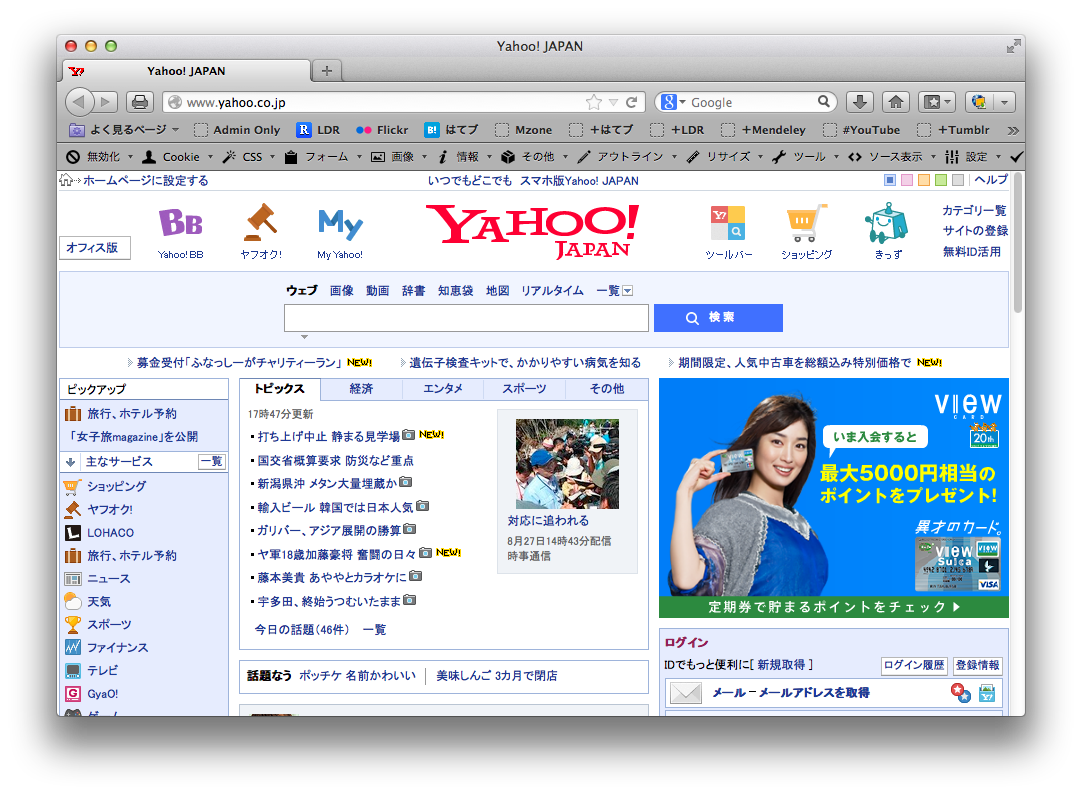
\includegraphics[height=7cm]{./yahoo_pc.png}
        \caption{Yahoo! Japanのトップページ}
        \label{yahoo_pc}
    \end{center}
\end{figure}

では、iPhoneではどうでしょうか。

\begin{figure}[H]
    \begin{center}
        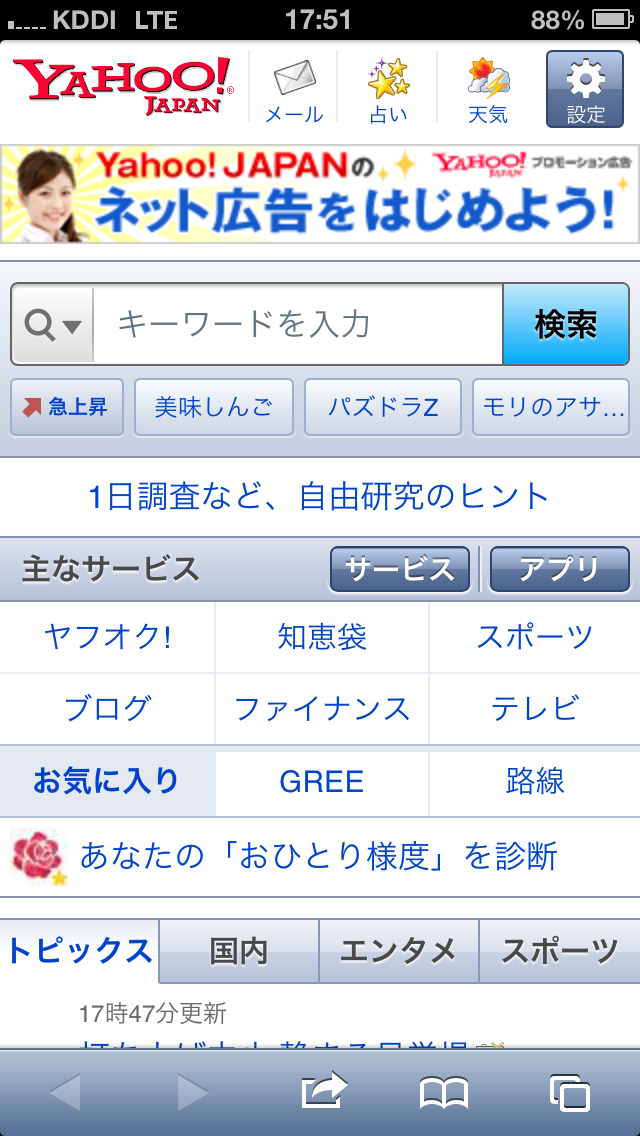
\includegraphics[height=5cm]{./yahoo_sp.png}
        \caption{Yahoo! Japanのトップページ}
        \label{yahoo_sp}
    \end{center}
\end{figure}

「なんだ、ブラウザにWebページが表示されているだけじゃないか!」と考えた人もいると思います。

そうです、それで正しいのです。HTMLはHypertext Transfer Protocol、即ちHTMLを転送するために生まれた通信の約束なのです。

\section{ブラウザ以外で見てみる}

さて、HTTPは「HTMLファイルを転送するための約束」となると、転送されたデータの使い道は、ブラウザである必要は全くないのです。こちらの画面、iPhoneを使った事がある人だと見覚えがありませんか?

\begin{figure}[H]
    \begin{center}
        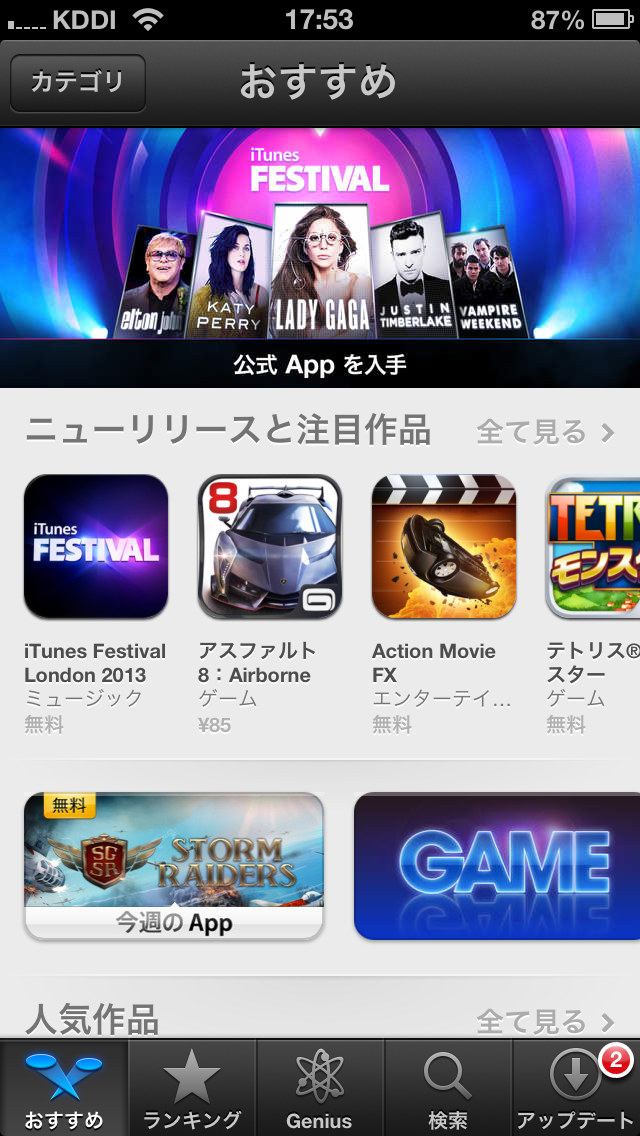
\includegraphics[height=5cm]{./app_store.png}
        \caption{App Store のページ}
        \label{yahoo_sp}
    \end{center}
\end{figure}

「あれ、ブラウザではないけど、どうして?」と思うかもしれません。それに、HTTPなのにHTMLページを転送していないじゃないか!と思われるかもしれません。

でも、これも実は正しいのです。現在、HTTPはHTMLファイルを転送するだけではなく、ネトゲ\footnote{ネットワークゲーム・オンラインゲーム}をはじめとしてネットワークを通じて情報をやり取りするためにも用いられています。

だから、HTTPは必ずブラウザだけで利用しなければならない、という事は無いのです。


\chapter{他にもあるプロトコル}

\section{どんなプロトコルがあるのだろう?}

インターネットで通信をするにあたって、プロトコルと言う通信の約束がある事がわかりました。その中に、HTTPがあります。

実は、HTTP以外にもプロトコルがあります。それは、何でしょうか?考えて、挙げてみましょう。

\begin{HUGE}
    \begin{itemize}
        \item 
        \item 
        \item 
        \item 
        \item 
        \item 
        \item 
        \item 
        \item 
        \item 
    \end{itemize}
\end{HUGE}

\section{どんなプロトコルがあるのだろう?}

いくつでてきましたでしょうか?ここで、よく使われるプロトコルを挙げてみます。

\paragraph{FTP\cite{RFC959}} File Transfer Protocol。ファイルをやり取りするためのプロトコル。最近はあまり使われなくなりました。

\paragraph{SSH\cite{RFC4250}} Secure SHell。暗号化通信を用いてサーバと直接接続するためのプロトコル。サーバをメンテナンスするとき等によく使われます。

\paragraph{SMTP\cite{RFC5321}} Simple Mail Transfer Protocol。メールを送信するためのプロトコルです。Thunderbirdからメールを送信する時、SMTPが使われているんですよ。

\paragraph{DNS\cite{RFC1034}} Domain Name System。「ドメイン」からインターネット上のIPアドレスを探す時に使うDNSサーバと通信するためのプロトコルです。とても身近なものですが、説明はまた別の機会に。

\paragraph{POP3\cite{RFC1939}} Post Office Protocol Version 3。メールサーバからメールを受信するためのプロトコルです。こちらも、皆さんよく使われていると思います。

\paragraph{NTP\cite{RFC958}} Network Time Protocol。時計合わせを行うためのプロトコルです。コンピュータの時計が合っているのは、このプロトコルの活躍があります。

\paragraph{TCP\cite{RFC793}} Transmission Control Protocol。先ほどまで挙げてきたプロトコルを支えるプロトコルです。正しいデータが流れるよう、通信の内容を管理しています。

\paragraph{UDP\cite{RFC768}} User Datagram Protocol。TCPの兄弟ですが、こちらはデータが正しく到達したかは管理しません。即時性を求めるデータを転送する時に使われる場合があります。


\chapter{どうやってやりとりしているの?}

\section{サーバとユーザエージェント}

皆さんはインターネット上に「サーバ」があることをご存知だと思います。また、サーバからデータを受け取る端末があります。HTTPではこれを「ユーザ エージェント」と呼びます。

さて、人同士で互いの意思を伝え合う時、会話をしますよね。多くの人は、それを「声」という形で行います。

では、「サーバ」と「ユーザ エージェント」の間では、どのような会話…コンピュータ同士ですから通信が行われているでしょうか?ちょっと考えて、吹き出しの中、および通信方向に矢印を書き込んでみましょう。


\begin{figure}[H]
    \begin{center}
        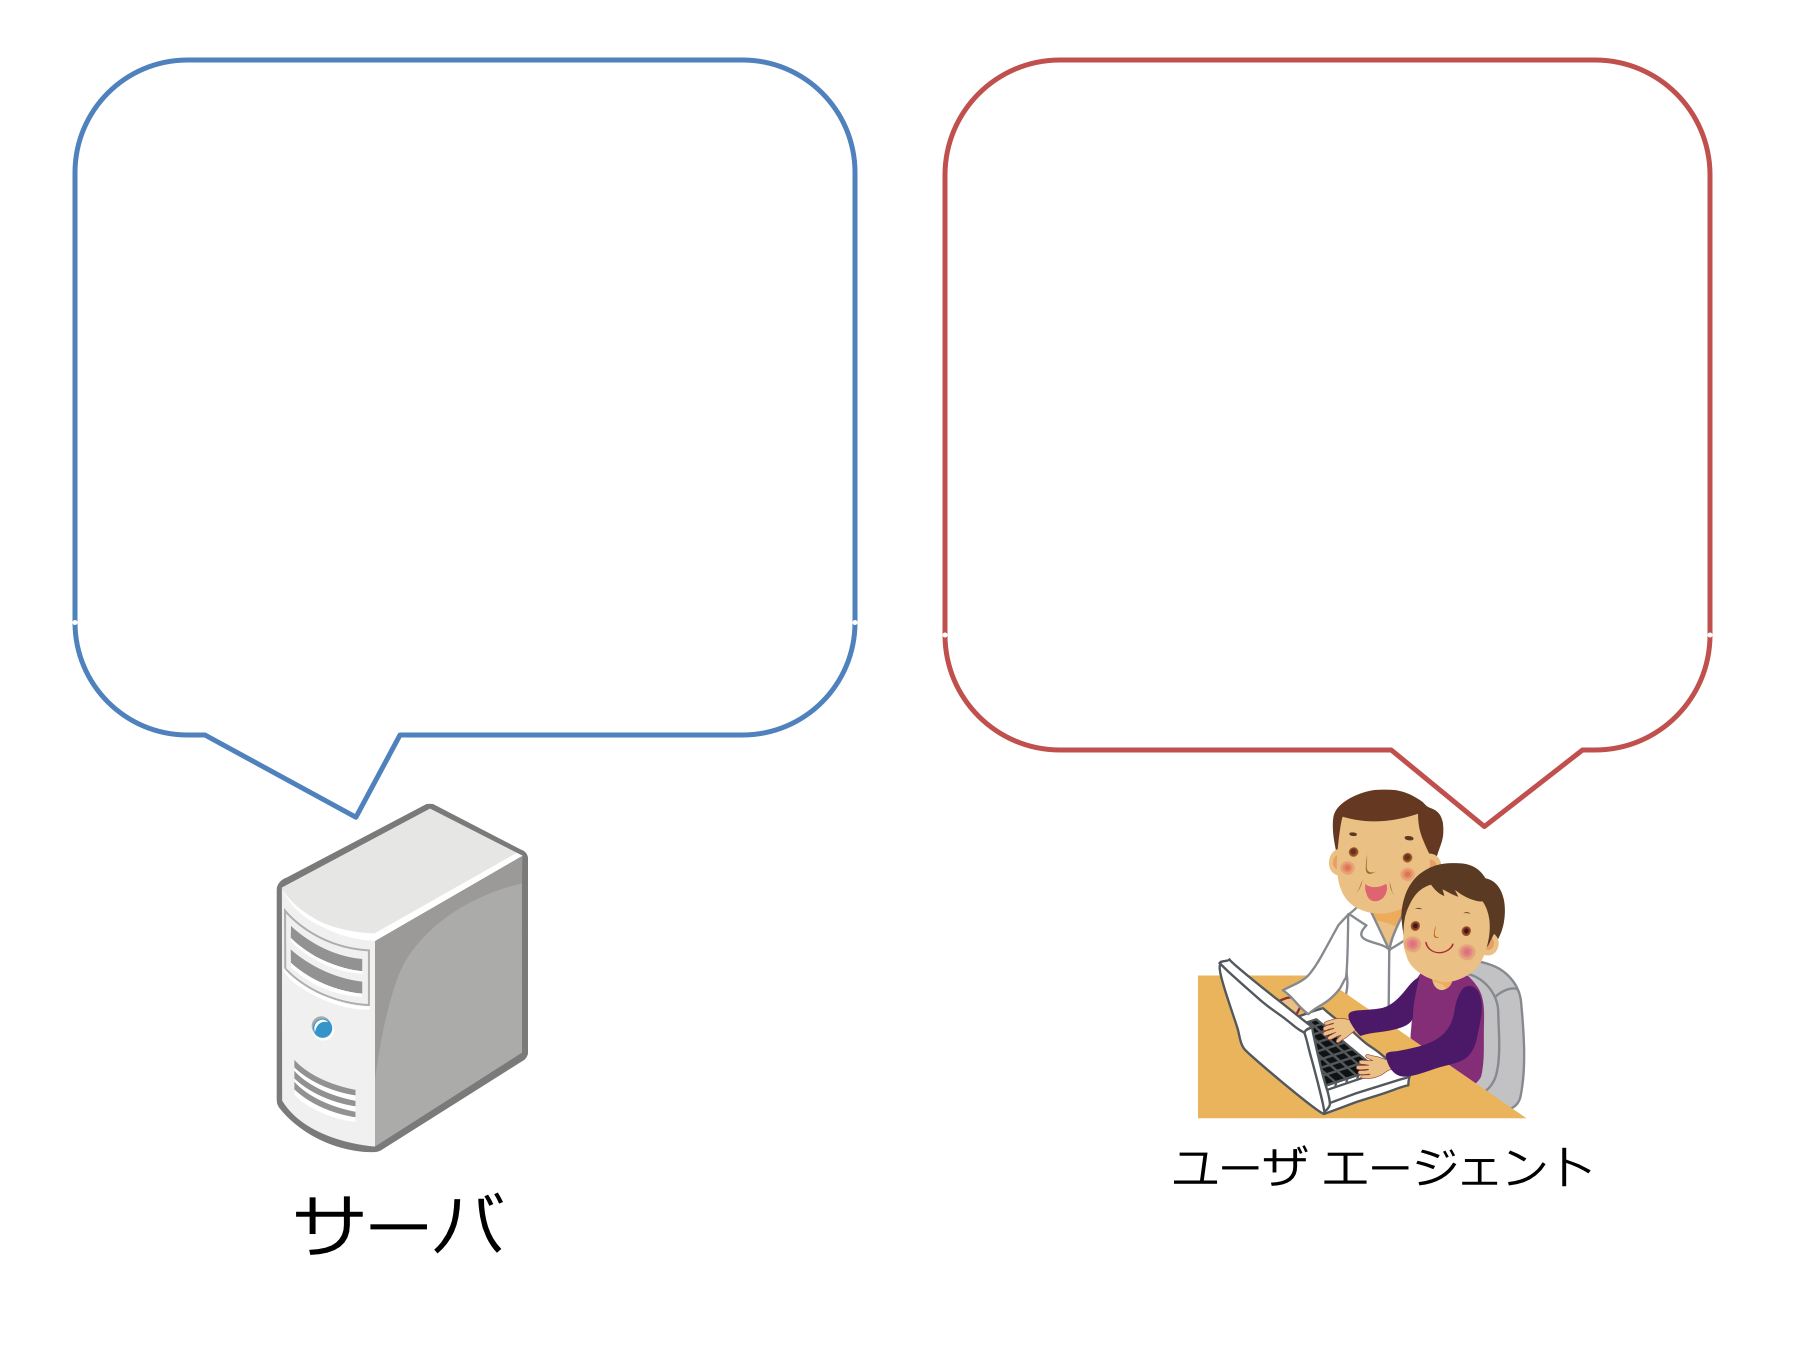
\includegraphics[height=9cm]{./req_res_1.png}
        \caption{どんな通信が行われているのでしょう!?}
        \label{req_res_1}
    \end{center}
\end{figure}

いかがでしょうか?みんなで見合わせて話し合ってみましょう。

\section{リクエストとレスポンス}

HTTPの通信は、次の2つの通信で説明する事ができます。

\begin{figure}[H]
    \begin{center}
        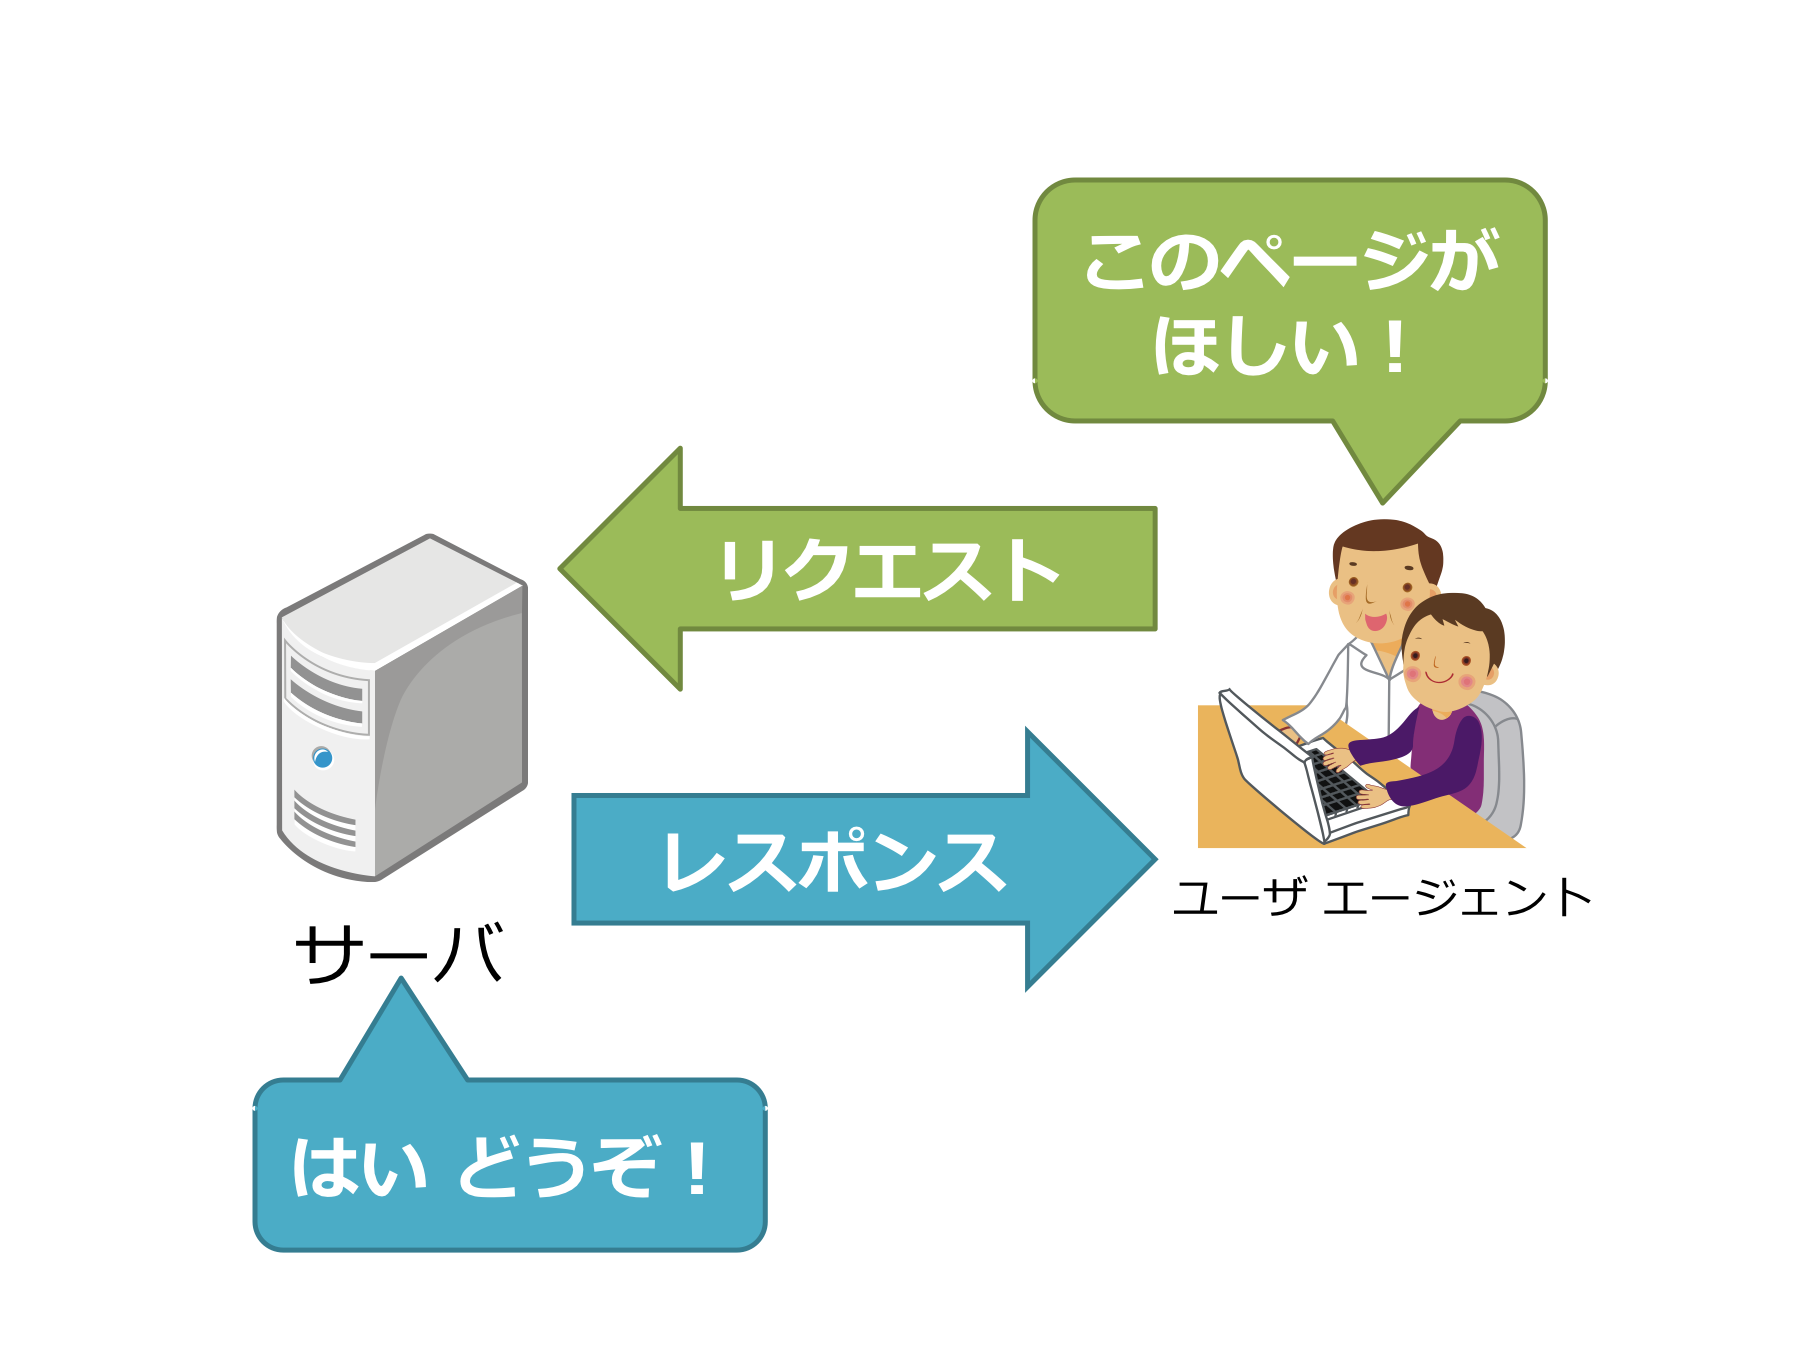
\includegraphics[height=7cm]{./req_res_2.png}
        \caption{リクエストとレスポンス}
        \label{req_res_2}
    \end{center}
\end{figure}

ユーザ エージェント側から発せられる通信を「リクエスト」(日本語: 要求)、サーバから返される通信を「レスポンス」(日本語: 回答)といいます。

これを、日常の会話のモデルに当てはめて考えてみましょう。

\begin{table}[H]
  \begin{small}
  \begin{center} 
	\caption{リクエストとレスポンス}
	\label{req_res_model}
	\begin{tabular}{|c||l|l|} \hline
		             & 人                        & HTTP通信 \\ \hline \hline
		リクエスト   & 「あなたは何歳ですか?」  & 「トップページをください」 \\ \hline
      	レスポンス   & 「32歳です」              & トップページのデータが届く  \\ \hline
	\end{tabular}
  \end{center}
  \end{small}
\end{table}

単純ですね。でも、これがHTTP通信の大切な基本です。


\chapter{通信の時に何がやり取りされているの?}

\section{実際に通信してみよう!}

いきなりですが、Windowsの「コマンドプロンプト」を開いて、サーバと通信してみましょう。

\begin{figure}[H]
    \begin{center}
        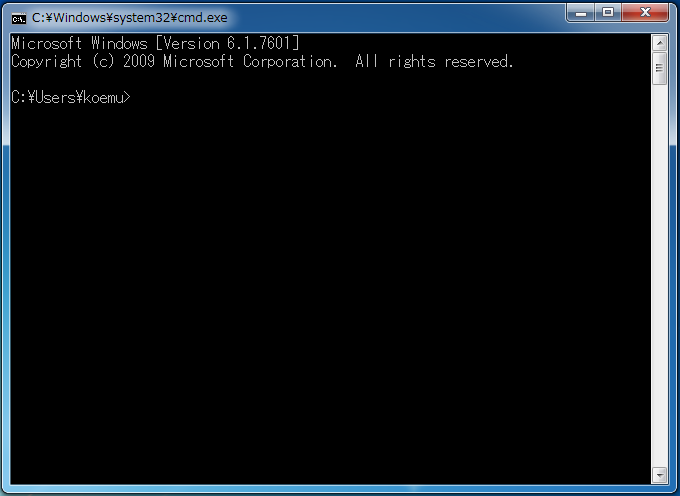
\includegraphics[height=5cm]{./cmd.png}
        \caption{ブラウザで表示}
        \label{browser}
    \end{center}
\end{figure}

上記の画面が開けたら、上記の文字を入力してEnterを押してください。

\begin{lstlisting}
C:¥> telnet www.koemu.com 8888
\end{lstlisting}    

続いて、次の文字が表示されるか確認してください。

\begin{lstlisting}
Trying 219.94.232.204...
Connected to www.koemu.com.
Escape character is '^]'.
\end{lstlisting}

そして、次の文字を入力します。文字が見えない人がいるかもしれませんが、目をつぶっていると思って、がんばって打ち込んでみてください!

\begin{lstlisting}
GET / HTTP/1.0
\end{lstlisting}

最後に、Enterを2回押したら…何がでるかを確かめてみてください。

\section{どのような通信が行われているのだろう?}

改めて、先ほど打ち込んだ内容について確認してみましょう。

最初に、以下の内容を打ち込みました。

\begin{lstlisting}
C:¥> telnet www.koemu.com 8888
\end{lstlisting}

これは、つなぐサーバのアドレスを入力しています。

次に、画面に次の情報が表示されました。

\begin{lstlisting}
Trying 219.94.232.204...
Connected to www.koemu.com.
Escape character is '^]'.
\end{lstlisting}

1行ずつ追いかけてみましょう。

1行目は、「Trying 219.94.232.204...」は「IPアドレス 219.94.232.204にあるサーバに接続を試みています。」です。

2行目は、「Connected to www.koemu.com.」は「www.koemu.comに接続しました。」となっています。うまく接続できたみたいですね。

3行目は、「Escape character is '\^]'.」→「エスケープ文字(特別な意味がある文字)は'\^]'(ESCキー)です」とでています。これは接続する事とは直接関係ありません。

そうです、ここで早速「リクエスト」と「レスポンス」のやり取りが行われているのです。初めに打ち込んだ文字が、サーバに接続しますというリクエスト、返ってきた3行の文字列がサーバからのレスポンスです。

続いて、次の文字を打ち込みました。

\begin{lstlisting}
GET / HTTP/1.0
\end{lstlisting}

これは、サーバに「ルートディレクトリ(フォルダの中の一番上にある所)にあるファイルが欲しい」というリクエストです。この書き方は、HTTPで定義された書き方に則っています。

そして、サーバから返ってきたレスポンスがこちら。

\begin{lstlisting}
HTTP/1.1 200 OK
X-Powered-By: Express
Content-Type: text/plain
Content-Length: 12
Connection: close

Hello World
Connection closed by foreign host.
\end{lstlisting}

8行のレスポンスが返ってきました。このレスポンスも、HTTPに則っています。

1行目、「HTTP/1.1 200 OK」ですが、これはサーバが「正しく処理できました」と返事をしています。200という数字は「ステータスコード」という名前があり意味もあるのですが、後ほど説明します。

2行目、「X-Powered-By: Express」は、サーバ側で「Express」というプログラムがこの処理を管理している事を示します。ただし、ユーザエージェントに対して意味があるレスポンスではありません。このようなレスポンスには、たいてい「X-」で始まる名前がついています。

3行目、「Content-Type: text/plain」は、コンテントタイプと言って、どのようなファイルをレスポンスとして返すかを示しています。今回はtext/plain、すなわち皆さんがプログラム等を作る時に書いているテキスト形式のデータである事を伝えてきています。

4行目、「Content-Length: 12」は、返すファイルのバイト数を示します。

5行目、「Connection: close」は、接続を終えた事を意味します。close以外もあるのですが、今回は説明を省略します。

6行目、ここが空白です。実は、この空白には意味があります。空白行手前までが「ヘッダ」といって、主にサーバがどのような処理をしたかを示す情報が含まれています。

7行目、「Hello World」とあります。これが、レスポンスとして返したいファイルの中身です。今回はテキスト形式ですので、そのままテキスト形式の"Hello World"という文字がでています。また、この長さは、4行目の「Content-Length」のバイト数と一致します。

8行目、「Connection closed by foreign host.」とありますが、これはサーバへ接続するためのソフトが発したメッセージで、レスポンスではありません。すなわち、レスポンスは1行前までとなります。

ここで知っていただきたい事があります。

\begin{itemize}
    \item HTTPには、リクエスト・レスポンス、どちらにも書き方の約束が決まっている。
    \item レスポンスの中身は、1行空けた手前をヘッダ、その先にリクエストされたデータが入っている。
\end{itemize}

\section{ブラウザでやってみよう}

先ほど、サーバとHTTPで通信した事を、ブラウザでやってみましょう。

Internet Explorerなどのブラウザを立ち上げて、次のURIを入力し、Enterを押してください。

\begin{itemize}
    \item http://www.koemu.com:8888/
\end{itemize}

その結果、次のページが表示されます。

\begin{figure}[H]
    \begin{center}
        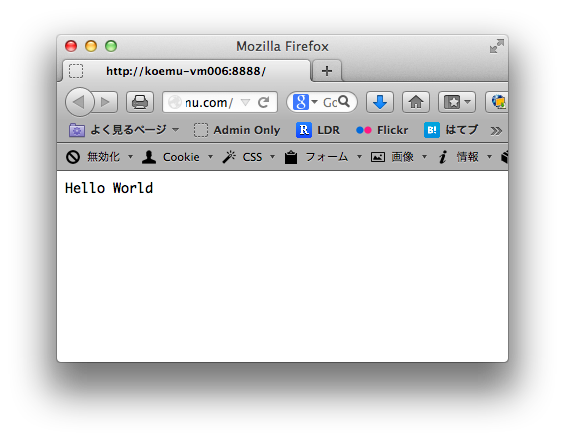
\includegraphics[height=7cm]{./browser.png}
        \caption{ブラウザで表示}
        \label{browser}
    \end{center}
\end{figure}

先ほど、コマンドプロンプトで確認した2回目のレスポンスの、5行目だけでて来ていると思います。そうです、ブラウザでは先ほど入力・受け取った内容のほとんどを、プログラムで処理しているのです。ブラウザは偉大ですね。

もちろん、自分自身でHTTPのリクエスト・レスポンスを自動処理するソフトウェアを作ることもできます。

\section{他のリクエストはどうだろう}

先ほどと同様に、サーバに接続してみます。

\begin{lstlisting}
C:¥> telnet www.koemu.com 8888
\end{lstlisting}    

そして、次の文字が表示されるか確認してください。

\begin{lstlisting}
Trying 219.94.232.204...
Connected to www.koemu.com.
Escape character is '^]'.
\end{lstlisting}

今回は、/(デフォルトのファイル)ではなく、"hoge.html"を取り出すリクエストを出してみましょう。

\begin{lstlisting}
GET /hoge.html HTTP/1.0
\end{lstlisting}

Enterを2回押したら…何がでるかを確かめてみてください。

\section{えっ、ページが無い?}

あれ…先ほどと様子が違いますね。

\begin{lstlisting}
HTTP/1.1 404 Not Found
X-Powered-By: Express
Content-Type: text/plain
Connection: close

Cannot GET /hoge.html
Connection closed by foreign host.
\end{lstlisting}

では、先ほどと違っている部分を確認して行きましょう。

1行目。「HTTP/1.1 404 Not Found」とあります。これは「ファイルが無い」事を意味しています。そう、"hoge.html"はサーバには存在しないのです。あと、ステータスコードが200ではなく404になっています。

6行目、本来ファイルの中身が表示される部分に「Cannot GET /hoge.html」、即ち「hoge.htmlを取得できません」と表示されています。これは、サーバ側であらかじめ定義された文章が返されるのが一般的です。

リクエストは必ずうまく行くものではなく、失敗する場合もある事を覚えておきましょう。

\section{エラーの状況をブラウザで確認してみよう}

では、エラーはブラウザではどのように見えるのでしょうか。

Internet Explorerなどのブラウザを立ち上げて、次のURIを入力し、Enterを押してください。

\begin{itemize}
    \item http://www.koemu.com:8888/hoge.html
\end{itemize}

その結果、次のページが表示されます。

\begin{figure}[H]
    \begin{center}
        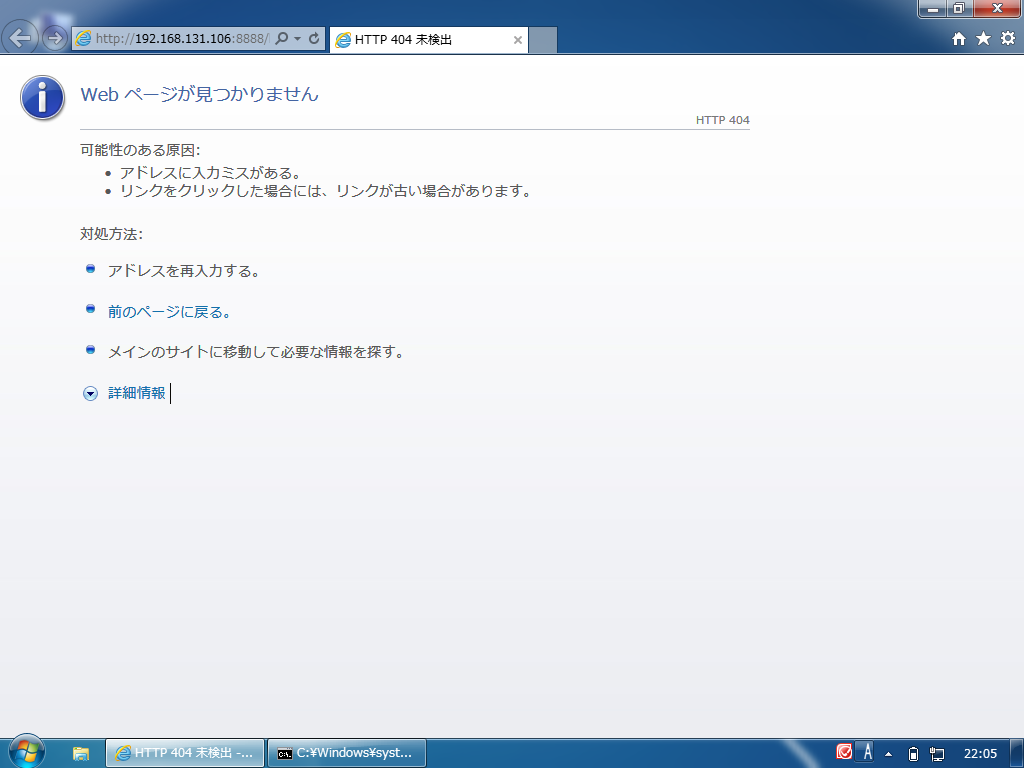
\includegraphics[height=7cm]{./404.png}
        \caption{エラーページがブラウザによって変更される例}
        \label{404}
    \end{center}
\end{figure}

先ほどのサーバのレスポンスでは「Cannot GET /hoge.html」とでていましたが、ブラウザにはでていません。これは、ブラウザがステータスコードを確認して、ユーザエージェントを利用している人がわかりやすいように代替のメッセージを出しているためです\footnote{「Cannot GET /hoge.html」と出してくれるブラウザもあります}。

\chapter{ステータスコードを知ろう}

\section{ステータスコードは3桁の数字}

さて、先ほどから200, 404などのステータスコードがでてきています。これは、サーバが、ユーザエージェントからのリクエストが正しく処理できたか否かを示す数値で、レスポンスの中に含まれています。

では、どのようなステータスコードが定められているでしょうか。自分がサーバの開発者だったらどのようなステータスコードを定めますか?または、ユーザエージェント側のソフトウェアを開発するなら、どのようなステータスコードが用意されているといいでしょうか。考えてみましょう。

\begin{HUGE}
    \begin{itemize}
        \item 
        \item 
        \item 
        \item 
        \item 
        \item 
        \item 
        \item 
        \item 
    \end{itemize}
\end{HUGE}

書き終わったら、友達同士で見せ合ってみましょう。

\section{代表的なステータスコード}

ステータスコードは、先にも述べた通り定義されています。

まず、数値には付番の原則が決まっています。

\begin{itemize}
    \item 100番台 --- 情報\footnote{あまり使われません}
    \item 200番台 --- 成功
    \item 300番台 --- ページが移動した
    \item 400番台 --- クライアント側のエラー
    \item 500番台 --- サーバ側のエラー
\end{itemize}

代表的なHTTPステータスコードを説明します。

\begin{itemize}
    \item 200 --- OK
    \item 301 --- Moved Permanently: ファイルが移動しました
    \item 307 --- Temporary Redirect: ファイルが一時的に移動しました
    \item 401 --- Unauthorized: 認証エラー (パスワードを間違えた等)
    \item 403 --- Forbidden: 許可が無い (特定の人のみアクセスできる場所)
    \item 404 --- Not Found: ファイルが無い
    \item 500 --- Internal Server Error: サーバ上でエラーが発生した
\end{itemize}

また、ステータスコードを見ると、プログラム側でも容易に成功・失敗を解釈する事もできます。プログラムを開発する時、エラーの有無を確認する時に使ってみてください。

全てのステータスコードは、RFCに定義されています。時間がある時に読んでみましょう。

\begin{itemize}
    \item http://www.studyinghttp.net/cgi-bin/rfc.cgi?2616
\end{itemize}

\chapter{きょうのまとめ}

では、今日学んだ事を復習しましょう。

\begin{enumerate}
    \item HTTPはインターネットを通じてファイルを転送する約束を定義したもの。
    \item 通信には「リクエスト」と「レスポンス」がある。
    \item 「リクエスト」には、主に取り出したいページファイルのアドレスを送っている。
    \item 「レスポンス」には、ページのデータの他に、リクエストの成否が含まれている。
    \item 「ステータスコード」はレスポンスに含まれており、リクエストがサーバ上でどのように処理されたかを知る最も単純な方法である。
\end{enumerate}

普段のTENTOの人とは違って、勉強っぽくなりちょっと大変だったかもしれません。

プログラムを書く事と同時に、ソフトウェアを取り巻く約束事の理解を深めて、より高度なソフトウェアが開発できるよう、取り組んで行きましょう!

今日の講義、おつかれさまでした。


\bibliographystyle{junsrt}
\bibliography{../library,../saito001,../rfc}


\end{document}
